\pagenumbering{arabic}

\chapter{Introduction} \label{introduction}

In compliance with ISO/IEC/IEEE 42010; see \textit{Clause 6}.\\
For the definitions of the viewpoints to be used, refer to Rozanski \& Woods’ “A Viewpoint Catalog” (R\&W) highlighted and commented.
Feel free to revise, extend, and refine the material that overlaps with your SRS.


\section{Purpose and objectives of FarmBot}

If you want to write unordered (bulleted) lists, you should use an "itemize" environment, where each list entry starts by using the \verb|\item| command, which also generates the bullet symbol.

\begin{itemize}
    \item Item1  
    \item Item2 
\end{itemize}

Numbered lists have the same syntax but use an "enumerate" environment: each entry must be preceded by the \verb|\item|, which will automatically generate numbers to label the item. 

For any citation, refer to it as \cite{younis2021hybrid}.

\section{Scope}

If you want to add any figure or diagram, you can use a figure environment.In Figure \ref{Fig:Example}

\begin{figure}[ht]
\centering
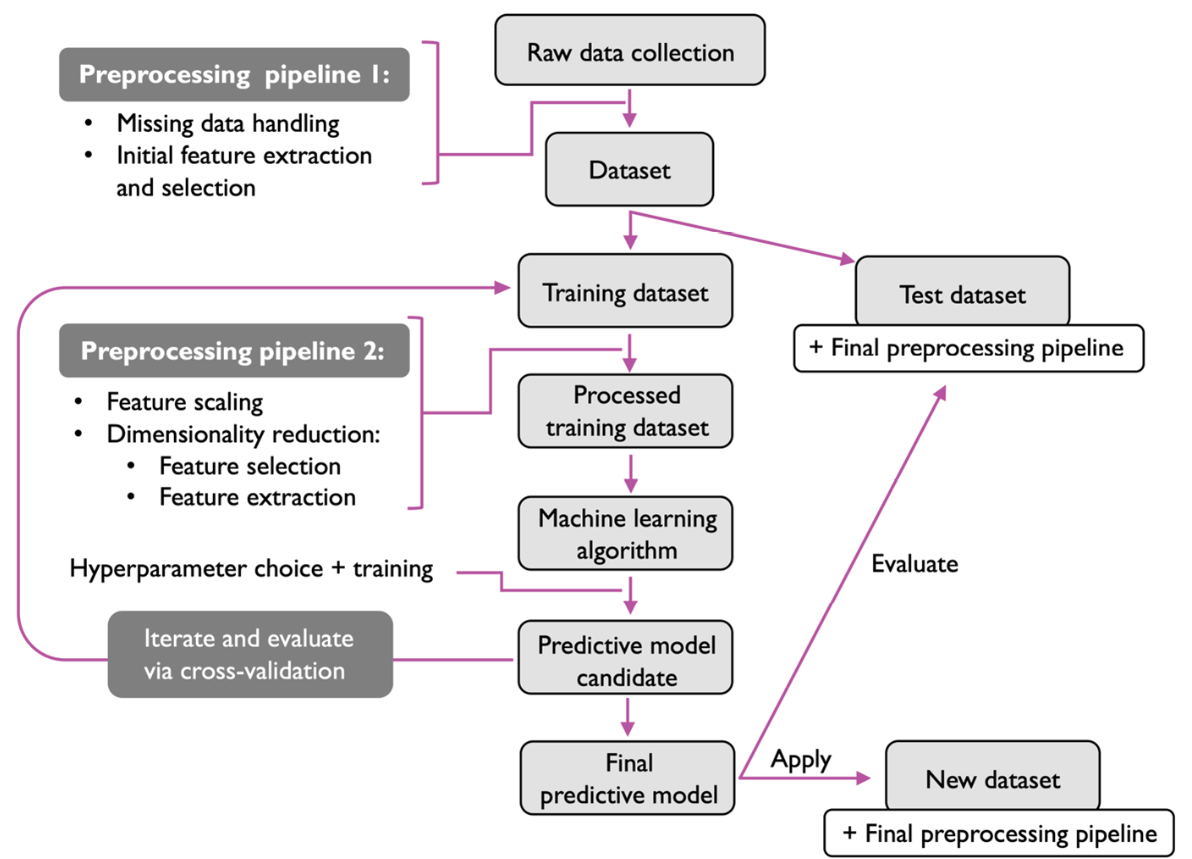
\includegraphics[width=.9 \textwidth]{Figures/ExampleFigure.png}
\caption{Example \label{Fig:Example}}
\end{figure}

\section{Stakeholders and their concerns}

For any citation, refer to it as \cite{younis2021hybrid}.

Terms are defined by means of the command \verb|\newglossaryentry| in the Glossary file. After you have defined the terms, to use them while you are typing your LATEX file use \verb| \gls{}|, \verb|\Gls| or \verb|\glspl| commands such as \gls{sad}. 




